\section{Introduction}
Hardware switches are a fundamental building block of the internet. The design of these switches is challenging, because they must support extremely fast line rates (up to hundreds of Gb/s for current Ethernet generations), while directing packets between arbitrary pairs out of a set of input and output ports.

One challenge switches must solve is how to schedule packets once their output port has been determined. A theoretically optimal solution to this is output queueing, where each packet is placed in a queue corresponding to its output port. Unfortunately, this is generally infeasible to implement in hardware, since it requires large amounts of redundant bandwidth to each output port. A simpler solution is input queueing, where packets are queued by their input port. This has another problem, head-of-line blocking: If the front packet in a queue can't be delivered to its output port yet, then all other packets behind it will be delayed even if their output ports are unavailable. The solution to this is virtual output queueing (VOQ), where packets are still buffered by their input ports, but in (logically) separate queues corresponding to each output. Then at each timestep, packets can be transferred from VOQs, subject to the constraint that no output receives more than one packet at a time, and no input sends more than one packet at a time.

Anderson et al \cite{anderson} frame the problem of choosing which VOQs to send from as a bipartite graph matching problem: finding the best possible matching between a set of input nodes and a set of output nodes, subject to a set of possible connections based on which packets are available to send. They propose an algorithm called Parallel Iterative Matching (PIM), which finds a maximal match (one which is not necessarily the best possible, but cannot be improved by adding a link) using a very simple algorithm which is amenable to hardware implementation. They evaluate this in simulations, showing that it is very likely to converge in a small number of iterations, and that it offers performance which is nearly as good as output queueing.

The PIM algorithm naturally gives equal priority to all possible input-output pairs. A natural question is to ask whether it is possible to modify the algorithm to support unequal bandwidth allocations. This is useful as a prerequisite to providing flow-level bandwidth guarantees. \cite{anderson} proposes an algorithm called Statistical Matching for this purpose, but does not evaluate its performance, and notes that it is restricted to allocating 72\% of the available bandwidth (the rest will be allocated evenly). Stiliadis and Varma \cite{stiliadis}\footnote{We reached out to Stiliadis and Varma with our preliminary reproduction results for comment, but have not heard back as of the time of this writing.} improve on this result with an algorithm called Weighted Probabilistic Iterative Matching (WPIM), which is simpler than Statistical Matching and is capable of allocating all available bandwidth in an arbitrary pattern. They show in their evaluation, again using a simulation, that WPIM has nearly identical latency performance to PIM, and much better performance than Statistical Matching. They also show that in the presence of misbehaving flows sending more than their allocation, it does a more consistent job than Statistical Matching of allocating bandwidth according to reservations.

\section{PIM, SM, and WPIM}
The three algorithms compared by Stiliadis and Varma all share a similar skeleton, but incorporate randomness and bandwidth guarantees in different ways.

\subsection{Probabilistic Iterative Matching (PIM)}
PIM works in a three step process, which can be iterated multiple times until a maximal or near-maximal match is found:

\begin{enumerate}
\item Each input will send a request to every output for which it has available traffic.
\item Each output will randomly choose one of the requests it received to grant.
\item Each input that had one or more of its requests granted will randomly choose one to actually send.
\end{enumerate}

The reason this must be iterated multiple times is because in the second step, multiple outputs may grant to the same input, meaning only one of those grants will actually result in a packet being sent. In the worst case, you can imagine a case where all inputs want to send to all outputs, but the outputs all grant to the same input in each iteration, meaning that only one packet is actually matched on each iteration. Even in this case, for an $N\times N$ switch the algorithm is guaranteed to find a maximal match after $N$ iterations, and in practice it's much faster because the randomness guarantees the worst case is unlikely.

A crucial part of the algorithm is that after one iteration through the matching process, the inputs and outputs that have been matched are removed from the process, and will not try to make conflicting matches.

\subsection{Statistical Matching (SM)}
As already mentioned, PIM will allocate bandwidth equally between all competing input-output pairs, and so is not suitable if bandwidth guarantees for particular input-output pairs are desired. SM was Anderson et al's attempt to address this problem, by incorporating weighted randomness into the matching process. Each input-output pair is assigned a number of credits proportional to its desired bandwidth allocation, and each iteration of the algorithm goes as follows:

\begin{enumerate}
 \item Each \begin{em}output\end{em} randomly chooses a single input to grant to, with probability proportional to its reservation.
 \item Each input randomly chooses up to one grant to accept, using a complex weighting system designed to ensure the probability of a match being made is proportional to the link's reservation.
\end{enumerate}

Because matches are initiated by the outputs, and each output only makes a single grant, there is a significant probability that a grant will be made to an input which has no traffic available to send to that output. This leads to the fact (acknowledged by Anderson et al) that SM can only allocate a limited fraction of the total bandwidth - roughly 63\% in a single iteration. Furthermore, although the algorithm can be iterated multiple times to increase the number of matches, these further iterations occur independently, without knowledge of what pairs were matched in the previous iteration, and so only a small proportion of the new matches found will actually be valid. This means that even with many iterations, only 72\% of the link throughput can be allocated fairly using SM. Anderson et al do not describe in detail why this limitation occurs, but we believe it has to do with the fact that matches are initiated by outputs, which do not have knowledge of which inputs have already matched a different output.

While this limited ability to allocate bandwidth seems like a very serious flaw, Anderson et al do describe a workaround to this in the first paragraph of section 5.2: "Any slot not used by statistical matching can be filled with other traffic by parallel iterative matching." Thus, full switch bandwidth can be achieved, at the cost of a slight degradation in fairness (since the last 28\% of bandwidth will be allocated without regard to bandwidth reservations).

\subsection{Weighted Probabilistic Iterative Matching (WPIM)}
WPIM is Stiliadis and Varma's attempt to solve the fair bandwidth allocation problem with a simpler and more efficient algorithm that SM. It works by dividing time into a series of frames, where each frame is long enough for the switch to transmit a fixed number of cells. Each input-output pair is guaranteed a certain number of cells in each frame, with the constraint that the allocations for all the pairs communicating with the same output must sum to the frame size or less. In addition, each output keeps track of how many cells have been transmitted from each input since the beginning of the latest frame.

Given this bookkeeping, the algorithm is very simple, and similar to PIM:

\begin{enumerate}
\item Each input will send a request to every output for which it has available traffic.
\item Each output will mask out any requests sent by an input which has already exceeded its allocation for the current frame.
\item Each output will randomly choose one of the remaining requests it received to grant.
\item Each input that had one or more of its requests granted will randomly choose one to actually send.
\end{enumerate}

In other words, traffic will be allocated randomly, except that once an input-output pair has exceeded its bandwidth allocation for the current frame it will be excluded from the matching process. If the allocations sum to less than the frame length and enough traffic is available, this guarantees that each input-output pair will receive its full bandwidth allocation every frame.

Finally, in cases where bandwidth is under-allocated, or flows are not sending their full allocated bandwidth, it's beneficial to allocate the spare capacity to flows that have traffic available exceeding their bandwidth allocation. Similarly to what Anderson et al suggest for SM, this is achieved by running normal PIM once WPIM is completed, filling in any gaps in the match and maximizing bandwidth utilization.

\section{Reproduction Approach}
In order to reproduce the results of both papers, we wrote a simulator in Python for input-buffered crossbar switches with VOQs. The simulation divides time up into equal slices, with one packet arriving and one packet leaving over each input/output port in each time slice. (This assumption is appropriate for the ATM networks that are the subject of the two papers, since they consist of cells of equal length.) Since we are not interested in modeling routing decisions, each packet is simply annotated with an input port and an output port, and is placed in the appropriate VOQ upon arrival at the switch. At each time step, after a scheduling decision is made, packets are removed from the appropriate VOQs, and statistics on latency and throughput are recorded.

The object representing the switch is sub-classed to implement different matching algorithms. In order to reproduce the comparisons of different algorithms from \cite{stiliadis}, three algorithms are necessary: PIM, Statistical Matching, and WPIM (described above). 

The trick part was implementing a statistical matching algorithm as ~\cite{anderson} was unclear on some points. First, the paper described $X$ as the allocatable bandwidth per link. We interpreted it as the size of the frame length which is mentioned in ~\cite{stiliadis}. Second, the paper did not explicitly mention what happens when the grant does not have the outstanding packet. In that case, we simply did not schedule any of the packets.

In order to reproduce the different traffic patterns used in the evaluations from the original papers, we wrote a variety of input generator classes, which run the switch's simulation for a prescribed number of timesteps, producing input traffic at each timestep based on the desired traffic pattern. Supported traffic patterns include the uniform traffic pattern used in evaluations for \cite{anderson}, a client-server pattern used for latency evaluations in \cite{stiliadis}, and a pattern also used in \cite{stiliadis} to model oversubscription of link bandwidth.

\section{Results}
\subsection{Reproduction of Anderson et al}
As a first test of our simulator and implementation of PIM, we began by reproducing Table I from Anderson et al, which showed what percentage of matches were found by running a certain number of iterations of PIM, compared to the number of matches found by allowing it to run until termination. Our results, shown in Table~\ref{tab:anderson_I}, very closely match the results from the source. The table reports our results, in terms of the load (fraction of VOQs with available packets to send when the matching is run), as well as the absolute percentage point difference between our result and their results. Our comparisons are of course limited to the number of significant digits that were presented in the original authors' table.

\begin{table}[]
\caption{Reproduction of Table I from Anderson et al: Percentage of maximal match found within K iterations (difference from original in parentheses)}
\hskip-1.2cm\begin{tabular}{@{}ccccc@{}}
     & \multicolumn{4}{c}{Number of iterations (K)} \\ \cmidrule(l){2-5} 
Load & 1         & 2        & 3         & 4         \\ \midrule
0.10 & 87\% (0.\%) & 99.7\% (-0.1\%) & 99.99\% (-0.01\%) & 100\% (0.00\%) \\
0.25 & 76\% (+1\%) & 97.6\% (0.0\%)  & 99.91\% (-0.06\%) & 100\% (0.00\%) \\
0.5  & 69\% (0.\%) & 93\% (0.\%)     & 99.4\% (-0.2\%)   & 99.95\% (-0.05\%) \\
0.75 & 66\% (0.\%) & 90\% (0.\%)     & 98.4\% (-0.2\%)   & 99.85\% (-0.12\%) \\
1.0  & 64\% (0.\%) & 88\% (0.\%)     & 97\% (0.\%)       & 99.7\% (-0.2\%)  
\end{tabular}
\label{tab:anderson_I}
\end{table}

For the another round of sanity check, we used our simulation tool to reproduce a figure from Anderson et al, as shown in Figure~\ref{fig:5-anderson}. It shows the average delay of the packet based on the number of iterations of PIM and the load on each input queues. It assumed a uniform traffic pattern. As can be seen, we were able to reproduce effectively identical results in our simulation.

\begin{figure}
    \centering
    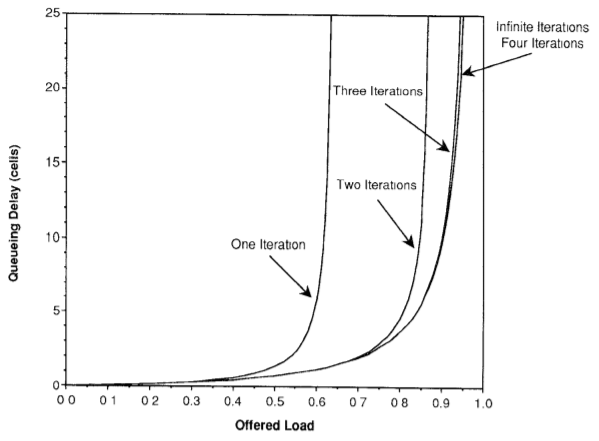
\includegraphics[width=\linewidth]{figures/anderson_fig5_original.png}
    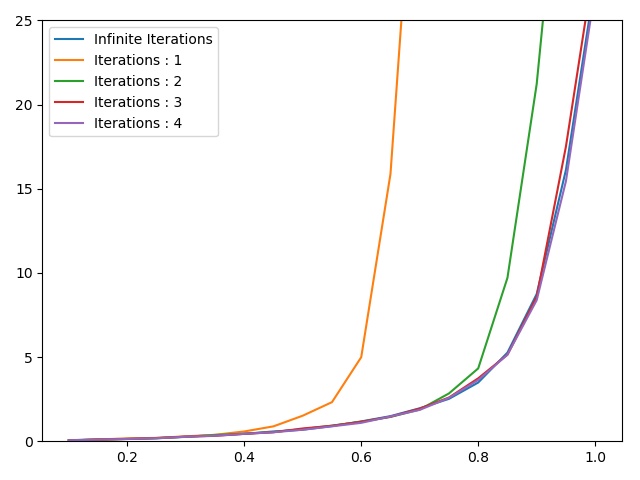
\includegraphics[width=\linewidth]{figures/anderson_fig5.png}
    \caption{Reproduction of Figure 5 from Anderson et al: Simulated performance of iterative matching with a uniform work load. Original (top) vs. reproduction (bottom).}
    \label{fig:5-anderson}
\end{figure}

\subsection{Reproduction of Stiliadis and Varma}

\subsubsection{Latency}

The first major result of Stiliadis and Varma is in Figure 4 from their paper, which compares the queueing latency of SM and WPIM. They simulate a "client-server" traffic model on a 16x16 switch, where four of the ports correspond to servers, and the other 12 correspond to clients, and the majority of the traffic flows from clients to servers and back. Each input-output connection is assigned bandwidth (in the SM or WPIM algorithm) proportional to the actual traffic on that connection, so none of the flows should end up bandwidth limited. Their results are shown, as well as our reproductions of the same, are shown in Figure~\ref{fig:4-stil}

\begin{figure}
    \centering
    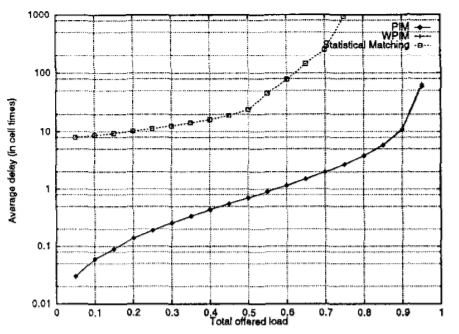
\includegraphics[width=\linewidth]{figures/stiliadis_fig4_original.png}
    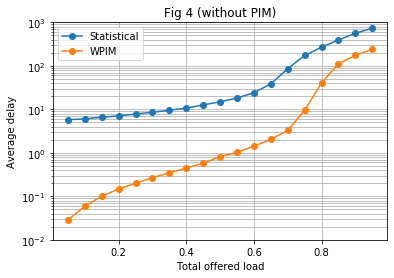
\includegraphics[width=\linewidth]{figures/stiliadis_fig4_no_pim.png}
    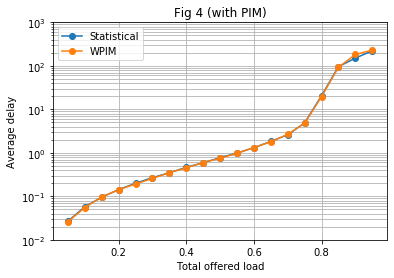
\includegraphics[width=\linewidth]{figures/stiliadis_fig4_pim.png}
    \caption{Figure 4 of Stiliadis and Varma - original, and our reproductions (with and without running PIM to fill in gaps left by SM)}
    \label{fig:4-stil}
\end{figure}

In the original results, SM has drastically higher queueing latency than PIM or WPIM. This is because the output-initiated matching of SM means that several cycles may go by before an input with traffic to send is selected by the output. When we implemented SM \begin{em}without\end{em} running a round of PIM to fill in gaps left by SM, we produced similar results, seen in the middle graph of Figure~\ref{fig:4-stil}. However, when we did use PIM to fill in gaps left by SM, the latency gap disappeared entirely, as seen at the bottom of Figure~\ref{fig:4-stil}.

Thus, we can see that the latency benefits of WPIM over SM disappear when SM is used in the context originally proposed by Anderson et al - accompanied by PIM to fill in any gaps not allocated by SM. In fairness to Stiliadis and Varma, the use of PIM in this way is only mentioned in passing in Anderson et al, and is not formally presented as a step in the SM algorithm, so the comparison is arguably justified when one is talking about the performance of SM in isolation.
\subsubsection{Fair Allocation}
The next major result of the paper is Figure 6 from the original paper, which compares how the three algorithms allocate scarce bandwidth between competing flows. The experiment setup involves four input ports all sending traffic to a single output port, with the inputs being allocated 10\%, 20\%, 30\%, and 40\% of the output bandwidth, respectively. The load on each input is varied from 5\% to 95\%, and the percentage of output bandwidth allocated to each input is shown on the graph. Note that for loads above 25\%, the total amount of inbound traffic is greater than the capacity of the output link, and so bandwidth allocation decisions must be made.

The results of this experiment for the WPIM, PIM, and SM algorithms are shown in Figure~\ref{fig:6-stil}, both the original graphs and our reproduced versions. As can be seen, PIM ignores the bandwidth allocations and divides bandwidth equally, while both WPIM and SM divide bandwidth approximately according to the assigned allocations. 

\begin{figure*}
    \centering
    \minipage{0.32\textwidth}
        \centering
        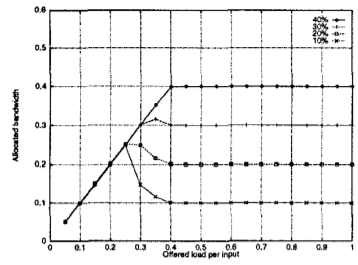
\includegraphics[width=\linewidth]{figures/stiliadis_fig6a_original.png}\\
        (a) WPIM original
    \endminipage\hfill
    \minipage{0.32\textwidth}
        \centering
        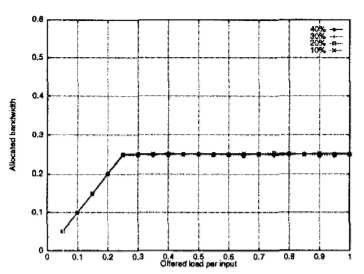
\includegraphics[width=\linewidth]{figures/stiliadis_fig6b_original.png}\\
        (b) PIM original
    \endminipage\hfill
    \minipage{0.32\textwidth}
        \centering
        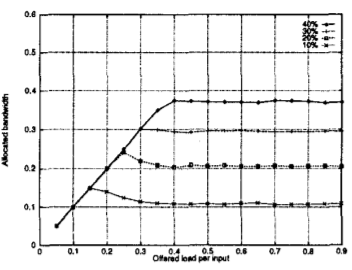
\includegraphics[width=\linewidth]{figures/stiliadis_fig6c_original.png}\\
        (c) SM original
    \endminipage\hfill
        \minipage{0.32\textwidth}
        \centering
        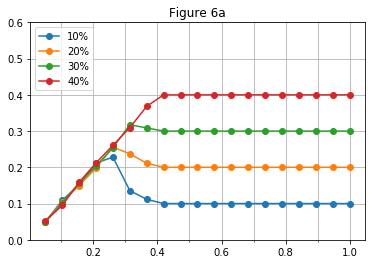
\includegraphics[width=\linewidth]{figures/stiliadis_fig6a.png}\\
        (d) WPIM reproduced
    \endminipage\hfill
    \minipage{0.32\textwidth}
        \centering
        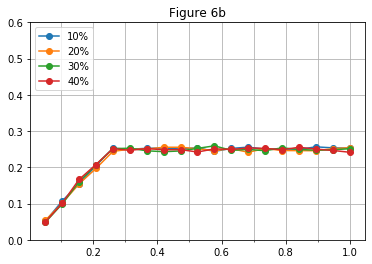
\includegraphics[width=\linewidth]{figures/stiliadis_fig6b.png}\\
        (e) PIM reproduced
    \endminipage\hfill
    \minipage{0.32\textwidth}
        \centering
        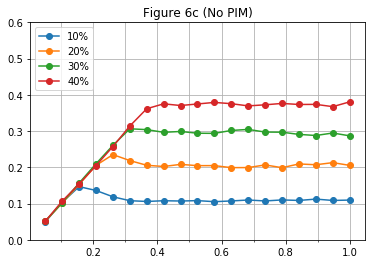
\includegraphics[width=\linewidth]{figures/stiliadis_fig6c_no_pim.png}\\
        (f) SM reproduced (no PIM)
    \endminipage\hfill
    \minipage{0.32\textwidth}
    .
    \endminipage\hfill
    \minipage{0.32\textwidth}
    .
    \endminipage\hfill
    \minipage{0.32\textwidth}
        \centering
        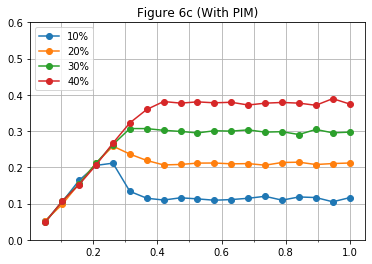
\includegraphics[width=\linewidth]{figures/stiliadis_fig6c_pim.png}\\
        (g) SM reproduced (with PIM)
    \endminipage
    \caption{Figure 6 of Stiliadis and Varma: Effective bandwidth allocated to four different connections, as a function of offered load per connection (WPIM vs. PIM vs. SM).}
    \label{fig:6-stil}
\end{figure*}

These graphs show that we were able to reproduce the fair allocation results essentially exactly. One thing we found key to our reproduction was using the correct number of iterations of SM: two iterations, as proposed by Stiliadis and Varma. With only a single iteration, SM would not allocate more to any flow than its bandwidth allocation, while as the number of iterations increased beyond two, SM got slightly better at allocating unused bandwidth at low loads to other flows.

The above SM reproduction graph was generated without running PIM to fill in gaps left by SM. If we add this step, then again we see that the performance of SM becomes more similar to that of WPIM, as seen in Figure~\ref{fig:6-stil}~(g). In particular, as one might expect, the final PIM step helps SM to re-allocate unused bandwidth at low loads, allowing each flow to receive nearly full bandwidth allocation up to a load of 0.25 per flow.

\section{Discussion}
We can draw several conclusions from this exercise. First of all, the use of simplified simulations in network research is a boon for reproducibility. We were able to make very precise reproductions of results from two 25 year old papers, even though we created our own simulator from scratch without access to any source code from the original papers. Had the research involved a physical switch or highly detailed simulation (e.g. an FPGA simulation of a hardware switch), this would have been a much more daunting task.

Second, small details in an algorithm can make very large differences to its performance. An easily overlooked detail in the presentation of the statistical matching algorithm, whether PIM is used to fill in gaps left by the statistical matching process, turns out to be key to evaluating its performance.

Third, there are other factors to consider when comparing algorithms than performance numbers. While SM used with PIM for gap-filling seems to have nearly identical performance to WPIM, this does not mean they are equally desirable. In our experience, WPIM was drastically easier to understand and to implement than SM, due to the complex probability calculations used in SM's matching process. In fact, it took us several attempts over a period of weeks to come up with what we believe to be a correct implementation of SM. Thus, in our opinion WPIM still deserves credit for being a much simpler version of a fair matching algorithm, one whose correctness is nearly trivial to verify.

\section{Reproducing the Reproduction}
All of the source code for our simulator and experiments is available in a public GitHub repo, available at:

\vspace{1em}
\url{https://github.com/torinmr/cs244-project}
\vspace{1em}

The README file of the repository contains instructions for setting up a Python virtual environment to mirror our own. Once this is done, the graphs and tables regenerated, by executing a Jupyter Notebook.\cite{jupyter}.

